

\begin{figure}[t]
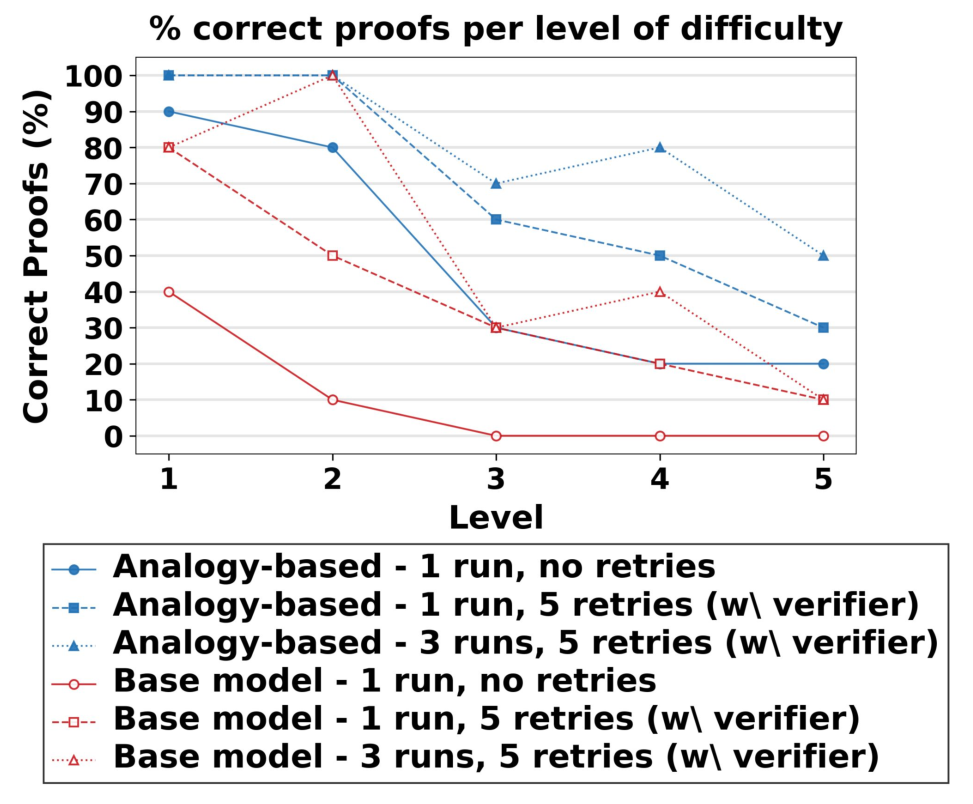
\includegraphics[width=0.48\textwidth]{latex/images/Experiments.pdf}
\centering
\caption{\% correct proofs per level of difficulty (50 samples, 10 per level). 
Our analogy-based method outperforms the o1 base model (non-analogy) in all settings. Analogy retrieval, verifier feedback, and multiple runs each significantly contributes to performance.
Our full pipeline (blue triangle) outperforms the baseline in every level, reaching an average aggregated accuracy of 80\%. Even without multiple runs (blue square), performance remains strong at 68\%, far exceeding the 10\% of the base model baseline (red hollow circle).
}
\label{fig:experiments_result}
\end{figure}




\begin{figure}[t]
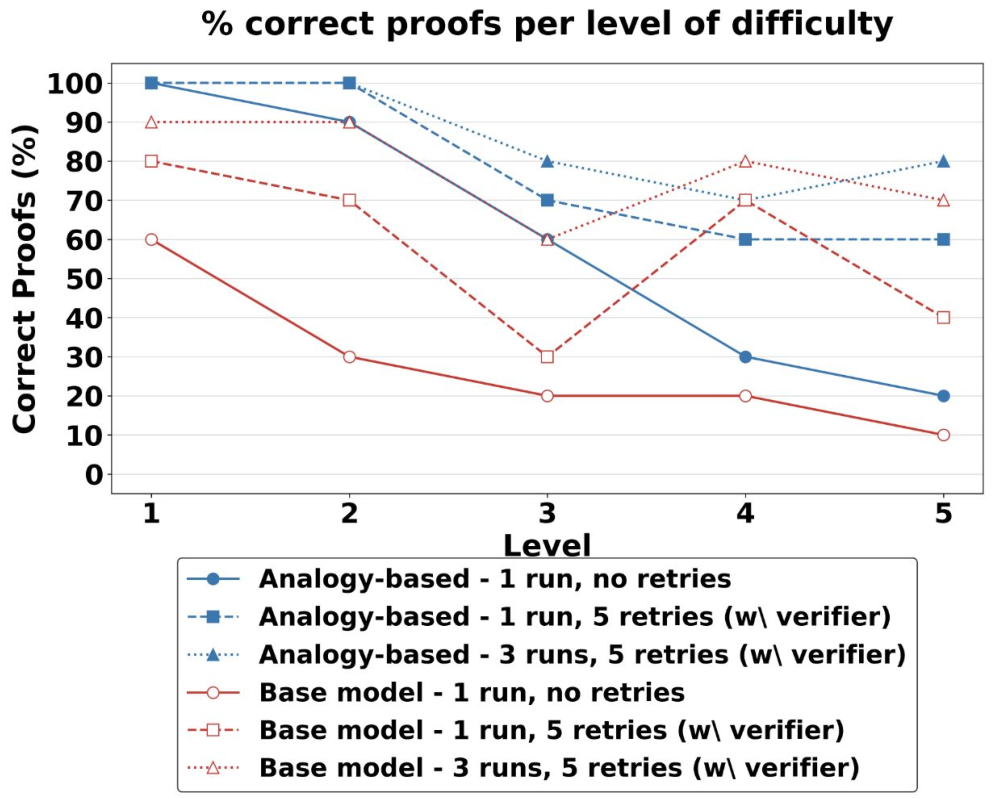
\includegraphics[width=0.48\textwidth]{latex/images/rq1_claude_cropped.pdf}
\centering
\caption{\% correct proofs per level of difficulty (50 samples, 10 per level). 
Our analogy-based method outperforms the Claude Sonnet-4.6 base model (non-analogy) in all settings. Analogy retrieval, verifier feedback, and multiple runs each significantly contributes to performance.
Our full pipeline (blue triangle) outperforms the baseline in every level, reaching an average aggregated accuracy of 86\%. Even without multiple runs (blue square), performance remains strong at 78\%, far exceeding the 28\% of the base model baseline (red hollow circle).
}
\label{fig:experiments_result_claude}
\end{figure}



\begin{figure}[t]
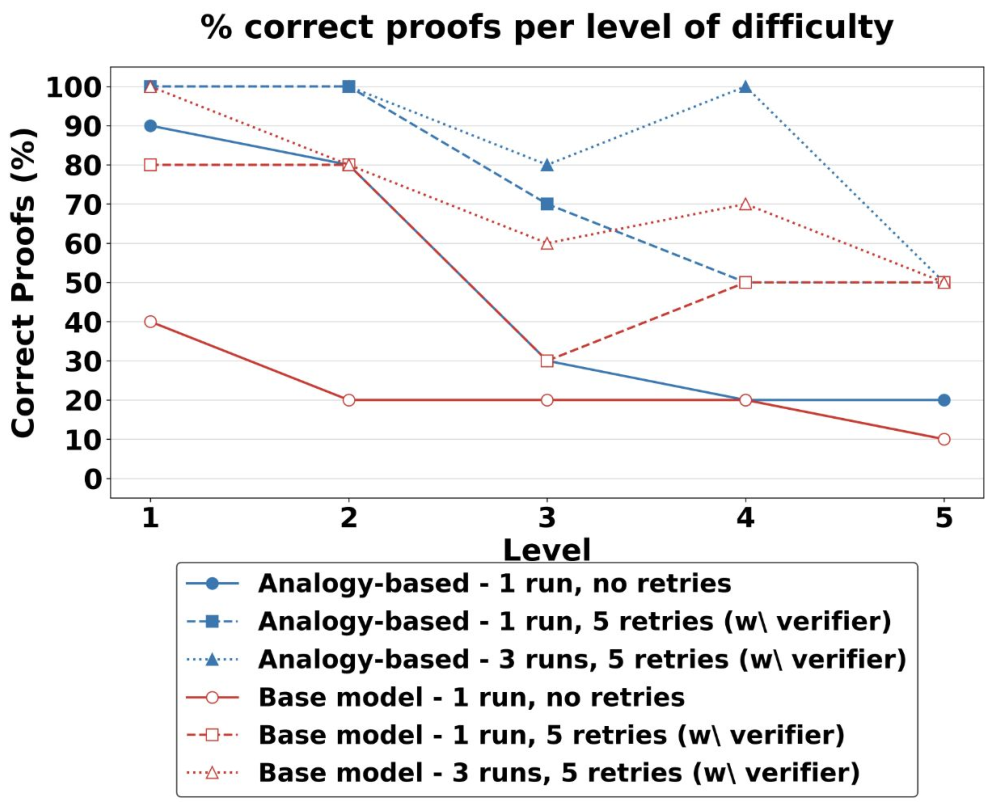
\includegraphics[width=0.48\textwidth]{latex/images/rq1_gemini_cropped.pdf}
\centering
\caption{\% correct proofs per level of difficulty (50 samples, 10 per level). 
Our analogy-based method outperforms the Gemini-Flash-2.5 base model (non-analogy) in all settings. Analogy retrieval, verifier feedback, and multiple runs each significantly contributes to performance.
Our full pipeline (blue triangle) outperforms the baseline in every level, reaching an average aggregated accuracy of 86\%. Even without multiple runs (blue square), performance remains strong at 74\%, far exceeding the 22\% of the base model baseline (red hollow circle).
}
\label{fig:experiments_result_gemini}
\end{figure}



\begin{figure}[t]
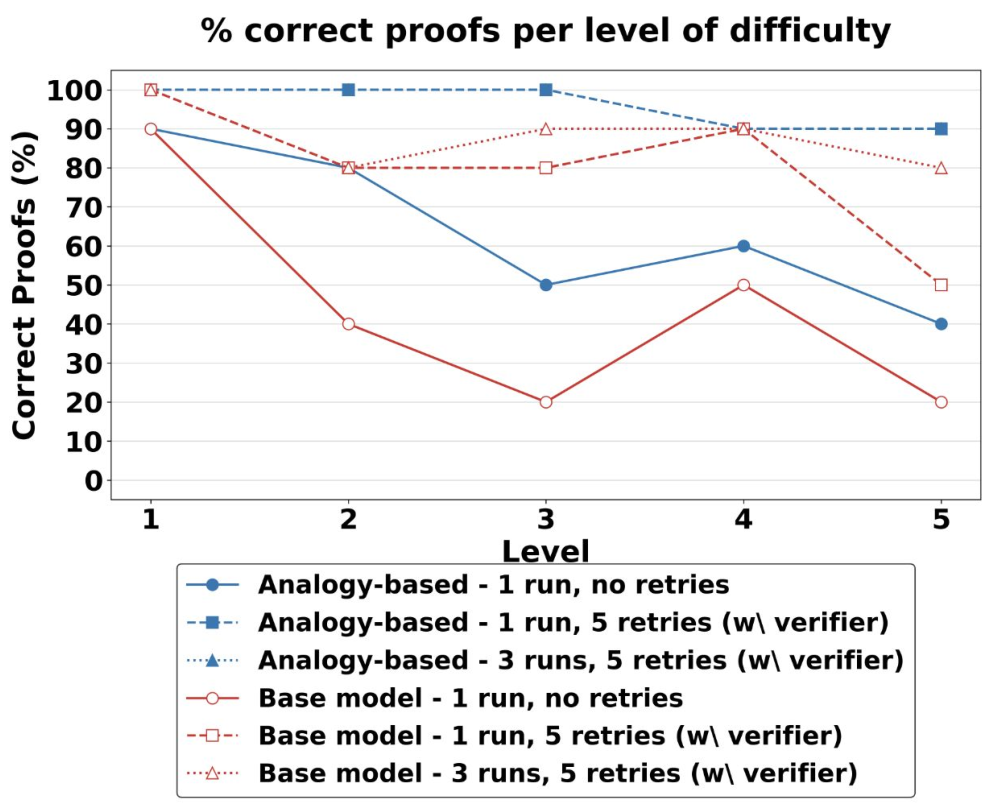
\includegraphics[width=0.48\textwidth]{latex/images/rq1_gpt5_cropped.pdf}
\centering
\caption{\% correct proofs per level of difficulty (50 samples, 10 per level). 
Our analogy-based method outperforms the GPT-5 base model (non-analogy) in all settings. Analogy retrieval, verifier feedback, and multiple runs each significantly contributes to performance.
Our full pipeline (blue triangle) outperforms the baseline in every level, reaching an average aggregated accuracy of 96\%. Even without multiple runs (blue square), performance remains stable at 96\%, far exceeding the 44\% of the base model baseline (red hollow circle).
}
\label{fig:experiments_result_gpt5}
\end{figure}



We provide additional details on the results and statistical analyses, focusing on the o1 model; similar trends are observed across other models.



Figure~\ref{fig:experiments_result} shows the results on o1 model for the different settings. 
We start by comparing our full pipeline (blue triangle: analogy + verifier, multiple runs with retries), to the most basic baseline (red hollow circle: non-analogy, no verifier, first run, no retries). Our full pipeline consistently outperforms the baseline at every level, achieving an average aggregated accuracy of 80\%. In contrast, the base model achieves an average of only 10\% (with 0\% accuracy on levels 3 and above).
This difference is statistically significant with $p=$5.82e-11 in the McNemar test at the 0.05 level (our method solved all problems the base model did, plus 35 others). 



To isolate the contribution of multiple runs, we also evaluated our model after a single run (blue square). This setting also substantially outperformed the base-model baseline, achieving an overall accuracy of 68\%,
with $p=$3.73e-09 in the McNemar test at the 0.05 level. % (solving the same 5 problems as the baseline plus 29 more). 
Thus, we conclude that our method significantly boosts the base model’s success rate in generating correct proofs, even without multiple runs.
See Figures~\ref{fig:experiments_result_gemini}, \ref{fig:experiments_result_claude}, and \ref{fig:experiments_result_gpt5} for the corresponding results on Gemini-Flash-2.5, Claude Sonnet-4.6, and GPT-5, respectively. 